% Layout similar to 
% https://admin-eguide.web.cern.ch/en/content/thesis-description-template
\documentclass{article}


% Define margins
\setlength{\topmargin}{-1.0cm}
\setlength{\oddsidemargin}{0.1cm}
\setlength{\textwidth}{16.5cm}
\setlength{\textheight}{23.0cm}

% language
\usepackage[english]{babel}

% graphics
\usepackage{pstool}                    % post-script editing from latex
\usepackage[dvips]{rotating,graphicx}  % use graphics 
\usepackage{float}                     % enables float options (positioning of elements)

% fonts
\usepackage[utf8]{inputenc}            % encode strings properly
\usepackage{lmodern}                   % loads latin-modern fonts
\usepackage{color}                     % use colors in text

% links
\usepackage{hyperref}
\hypersetup{
            %backref,  % already set somewhere
            pdfpagemode=UseOutlines ,
            linkcolor=[RGB]{0,51,160}, % blue,
            citecolor=[RGB]{0,51,160}, % blue,
            urlcolor=[RGB]{0,51,160}, % blue,
            % hyperfigures=true,  % already set somewhere
            colorlinks=true}


% other styles
\usepackage{enumitem}  % helps to make smaller dots in enum
\usepackage{latexsym}

% math
\usepackage{siunitx}                        % use si units with \si{unit} or \SI{#}{unit}
\usepackage{amsmath}                        % math package
\usepackage{mathtools}                      % allows mulit-column cases*
\usepackage{bm}                             % bold math symbols

% Define header and footer
\usepackage{lastpage}
\usepackage{fancyhdr}
\pagestyle{fancy}
\fancyhf{}
\rhead{\textbf{\textit{Adja Team}} }
\lfoot{\textbf{\textit{Page \thepage/\pageref*{LastPage}}}}
\renewcommand{\footrulewidth}{0.7pt}
\renewcommand{\headrulewidth}{0.7pt}

% tables
\usepackage{multirow}       % allows multiple rows put into one
\usepackage{booktabs}       % hline extensions like \toprule \bottomrule \midrule 
\usepackage{makecell}       % multiline cells
\usepackage{array}

% references
\usepackage{cite}
\usepackage[nameinlink,capitalize]{cleveref}  % easy referencing

% Fill in the names:
\newcommand{\StudentName}{Max Musterman}
\newcommand{\UniSupervisorName}{Prof. Dr. Dr. Goodman}
\newcommand{\CernSupervisorName}{Dr. Okayman}

\begin{document}

% magyar címoldal

\begin{center}
\vspace*{15\baselineskip}

{\huge \textbf{Imitációs tanulás a DuckieTown környezetben DAgger felhasználásával}}

\vspace*{3\baselineskip}

\begin{large}
\vspace*{2\baselineskip}

\vspace*{2\baselineskip}

Csapat:

\vspace*{\baselineskip}

Kovács Boldizsár - GVJY8E

\vspace*{\baselineskip}

Schneider Marcell - DBGYVI

\vspace*{\baselineskip}

Talpos Norbert - Q2H4XB

\vspace*{\baselineskip}

Virág József Ádám - U7KC0P

\vspace*{\baselineskip}

\end{large}
\end{center}
\pagebreak

% angol címoldal

\begin{center}
\vspace*{15\baselineskip}

{\huge \textbf{Imitation Learning in the DuckieTown environment with DAgger}}

\vspace*{3\baselineskip}

\begin{large}
\vspace*{2\baselineskip}

\vspace*{2\baselineskip}

Team:

\vspace*{\baselineskip}

Kovács Boldizsár - GVJY8E

\vspace*{\baselineskip}

Schneider Marcell - DBGYVI

\vspace*{\baselineskip}

Talpos Norbert - Q2H4XB

\vspace*{\baselineskip}

Virág József Ádám - U7KC0P

\vspace*{\baselineskip}

\end{large}
\end{center}
\pagebreak

% magyar abstract

\section*{Kivonat}
\large
2021-ben alig-alig lehet olyan mérnöki területet találni, amin a deep learning a megszokott paradigmákkal szembe menve ne tudna javulást elérni.
Az egyik legjellemzőbb ilyen terület az autóipar. A számítási teljesítmény növekedése és a deep learning fejlődése révén lehetőség nyílt az önvezető autók rohamos fejlődésére. Ezek fejlesztésében alapvetően két fő irányzat létezik: a Reinforcement Learning, amikor a modell egy szimulált környezetben tanul a reward function-t próbálja maximalizálni, illetve az Imitation Learning, amikor egy expert viselkedését próbálja megtanulni, és azt általánosítani.
Ezutóbbihoz szükség van a szimulált környezetben az expertre, illetve szükséges kiegészíteni a DAgger algoritmussal, ami azt teszi lehetővé, hogy a modell olyan helyzeteket is megtanulhasson az experttől, amiket egyébként nem látna tőle (például hogyan kell visszajönni az útra).
A házi feladatunkban az Imitation Learning+DAgger algoritmust dolgoztuk ki a DuckieTown környezetben.

% angol abstract

\vspace*{2\baselineskip}
\vspace*{2\baselineskip}
\vspace*{2\baselineskip}

\section*{Abstract}
Nowadays one can hardly find a field in engineering where deep learning couldn’t make an improvement opposed to the regular techniques.
One of the most well-known field is the automotive industry. The increase in computation power and the advances in deep learning made possible a breakthrough in making self-driving cars. There are two main branches of development in this field: Reinforcement Learning, in which the model learns by trying to optimize a reward function in the simulation environment, and Imitation Learning, whose goal is to try to clone the behaviour of an expert in the environment.
To make Imitation Learning a viable alternative, we need to complement it with the DAgger algorithm, which makes it possible to not only teach the model the optimal situations the expert would normally encounter, but the recoveries too.
In this homework we implemented the Imitation Learning+DAgger algorithm in the DuckieTown environment.

\pagebreak

% bevezető

\section*{Introduction}
In our project, we worked in a Duckietown environment to construct an AI model in the field of autonomous driving and imitation learning. At first, we preprocessed images by cropping and resizing them and then  we constructed a model consisting of three convolutional layers. The parameters of the layers have benn hyperparameter-optimized and we also used the Dagger-algorithm (an algorithm highly recommended for imitational training) to train our model through a Dagger expert (teacher). Our model will be able to determine the ideal steering (in radian) and speed (e.g. a two-element vector as the output) of the driven car according to the current observed image.

\vspace*{2\baselineskip}

%tématerület ismertetése, korábbi megoldások

\section*{Review of field and previous solutions}

There are various research projects conducted in the field of autonomous driving. Some of them include the thrilling environment of DuckieTown. Our project is set in the DuckieTown environment and make use of the imitation learning technique.

The field of imitation learning means learning algorithms designed to observe proper operation of functioning and thus educate the model. In other words, the imitation learning means the presence of a supervised agent providing the learner with data.

In the field of our project, the teaching means showing our model some training data consisting of proper driving pictures and corresponding driving actions, and then the main objective of our model is to predict an appropriate driving action.

The utilised methodology of our project contains the DAgger (data aggregation) algorithm. It trains the model on all the previous data collected by the agent. The driving data is created by the DAgger-expert. Of course, there are some other algorithms like Behavioral Cloning, GAIL and DAgger-extensions such as Ensemble DAgger and Reward-Guided DAgger.

During our examination of self-driving cars in DuckieTown environment, enormous advantage had been taken of a Scientific Students' Associations (TDK) research paper written by Zoltán Lőrincz, so that article is to be considered to be of paramount importance of the project.

% rendszerterv

\pagebreak

\section*{Network Architecture}
We use a 2d convolutional network with 3 convolutional layers, Leaky ReLU activation function, batch normalization, and max pooling. After that we flatten the output from the last convolutional layer and put the inputs through a dense layer with 12000 neurons. This layer uses ReLU activation, regularization and dropout. The output is a 2 element vector, whose entries are the velocity and the steering angle.


\begin{figure}

  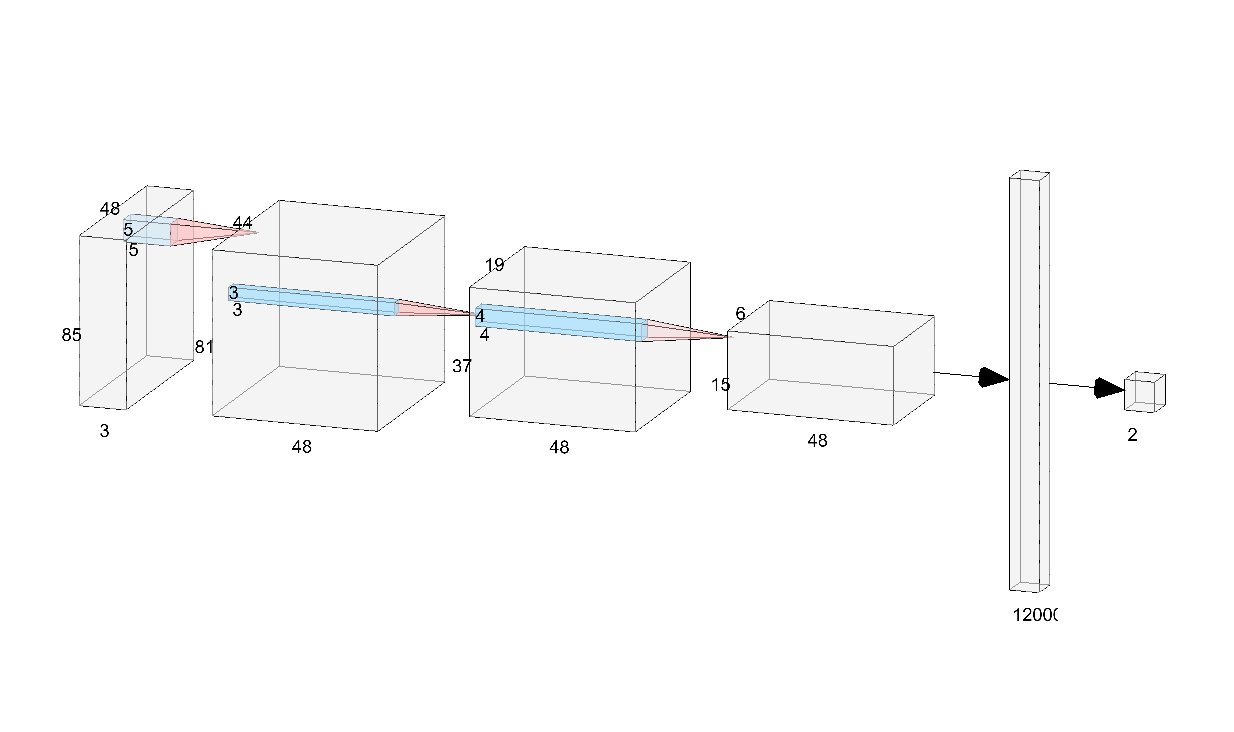
\includegraphics[width=\linewidth]{convnet.png}
  \caption{The architecture of the network}

\end{figure}

%adatok beszerzése, előkészítése
\section*{Obtaining and preprocessing data}

For the training, data were obtained in two ways. We used the DuckieTown environment's auto driver/expert, and we also drove a car ourselves using a keyboard. From these drives we extracted 3 things at each step. A picture, and the forward and sideways acceleration of the car. With this data we planned to teach.

Most of the information in the pictures was not considered useful, so we processed it in advance to make the teaching easier to work with. We used HSV image processing, which allowed us to separate the different colours from each other, and to minimise noise in the process. This made the asphalt almost completely black, as well as the lane divider yellow, and the road edge grey.

In addition, we have cropped the top of the images because we didn't think the sky was important, and we have also reduced the size of the images because they show the terrain well in a smaller image, but this makes teaching much faster as the size of the images is reduced.

This also helped the scanning of the data, as tens of thousands of images take up less than 40 MB.


\vspace*{2\baselineskip}

% megvalósítás

\section*{Implementation}
% TODO

\vspace*{2\baselineskip}

% jövőbeli tervek

\section*{Future plans}
% TODO
\pagebreak

% hivatkozások

\section*{References}
\vspace*{1\baselineskip}

Duckietown official website:
\\
\url{https://www.duckietown.org/}
\vspace*{1\baselineskip}

Duckietown baseline DAgger algorithm.
\\
\url{https://docs.duckietown.org/DT19/AIDO/out/embodied_il_sim_dagger.html}
\vspace*{1\baselineskip}

Duckietown-world.
\\
\url{https://github.com/duckietown/duckietown-world}

\vspace*{1\baselineskip}

Ian Goodfellow and Yoshua Bengio and Aaron Courville, „Deep Learning”, MIT Press, 2016

\vspace*{1\baselineskip}
Chigozie Enyinna Nwankpa, Winifred Ijomah, Anthony Gachagan, and Stephen Marshall, “Activation Functions: Comparison of Trends in Practice and Research for Deep Learning”, CoRR, arXiv: 1811.03378, pp. 8, 2018
\vspace*{1\baselineskip}
Wu Jianxin. "Introduction to convolutional neural networks.", National Key Lab for Novel Software Technology, pp. 11-23., 2017
\vspace*{1\baselineskip}
\vspace*{1\baselineskip}

Keras official website:
\\
\url{https://keras.io/}
\vspace*{1\baselineskip}

Keras Tuner tutorial:
\\
\url{https://www.tensorflow.org/tutorials/keras/keras_tuner}
\vspace*{1\baselineskip}

Deep Learning Wizard:
\\
\url{https://www.deeplearningwizard.com/}
\vspace*{1\baselineskip}

Zoltán Lőrincz, Imitation Learning in the DuckieTown Environment
\\
\url{http://tdk.bme.hu/VIK/DownloadPaper/Imitacios-tanulas-a-Duckietown-kornyezetben}


\begin{center}
\begin{tabular}{ | m{15em} | m{3em}| }
  \hline
  Name of the hyperparameter & Value  \\
  \hline
  \hline
  conv 1 filter & 80  \\
  \hline
  conv 1 kernel & 7 \\
  \hline
    conv 2 filter  & 64 \\
  \hline
    conv 2 kernel & 7 \\
  \hline
    conv 3 filter  & 48 \\
  \hline
    conv 3 kernel & 7 \\
  \hline
    dropout & 0.3 \\
      \hline
    learning rate & 0.001 \\
    \hline
\end{tabular}
\end{center}

\pagebreak

\clearpage
\end{document}
